\documentclass[a4paper,10pt]{article}
\usepackage[utf8]{inputenc}
\usepackage{subcaption}
\usepackage{amsmath}
\usepackage{pgfplots}
\usepackage{float}
\usepackage[parfill]{parskip}
\usepackage{siunitx}
\sisetup{detect-all}

%opening
\title{Měření Dopplerova jevu}
\author{Tomáš Kysela}
\date{29/11/2022}

\begin{document}

\maketitle

\section{Použité veličiny}

\begin{tabular}{l l l}
 $f_0$ & frekvence vysílače & [\si{\hertz}]\\
 $f$ & frekvence na přijímači & [\si{\hertz}]\\
 $v$ & rychlost vysílače & [\si{\meter\per\second}]\\
 $c$ & rychlost světla & [\si{\meter\per\second}]\\
 $t$ & teplota v místnosti & [\si{\celsius}]
\end{tabular}

\section{Známé hodnoty}

\begin{tabular}{l l}
 $t = 23.2\ \si{\celsius}$ & teplota v místnosti\\
 $c = (331.06 + 0.61t = 345.212)\ \si{\meter\per\second}$ & rychlost světla \\
\end{tabular}

\section{Závislost $f$ na $v$}
\subsection{Naměřené hodnoty}
\begin{table}[H]
    \centering
    \begin{minipage}{0.32\textwidth}
     \centering
     \begin{tabular}{|c|c|}
        $v\ [\si{\meter\per\second}]$ & $f\ [\si{\hertz}]$ \\ \hline
        0 & 39059 \\
        0 & 39060 \\
        0 & 39059 \\
        0 & 39061 \\
        0 & 39060 \\
        0 & 39060 \\
        0 & 39060 \\
        0 & 39060 \\
        0 & 39060 \\
        0 & 39060 \\
     \end{tabular}
    \end{minipage}
    \begin{minipage}{0.32\textwidth}
     \centering
     \begin{tabular}{|c|c|}
        $v\ [\si{\meter\per\second}]$ & $f\ [\si{\hertz}]$ \\ \hline
        0.181 & 39080 \\
        0.194 & 39082 \\
        0.201 & 39081 \\
        0.185 & 39081 \\
        0.191 & 39081 \\
        0.201 & 39082 \\
        0.196 & 39081 \\
        0.193 & 39081 \\
        0.210 & 39083 \\
        0.203 & 39082 \\
     \end{tabular}
    \end{minipage}
    \begin{minipage}{0.32\textwidth}
     \centering
     \begin{tabular}{|c|c|}
        $v\ [\si{\meter\per\second}]$ & $f\ [\si{\hertz}]$ \\ \hline
        -0.206 & 39037 \\
        -0.206 & 39038 \\
        -0.210 & 39037 \\
        -0.204 & 39037 \\
        -0.205 & 39037 \\
        -0.202 & 39037 \\
        -0.208 & 39037 \\
        -0.217 & 39036 \\
        -0.213 & 39036 \\
        -0.217 & 39036 \\
     \end{tabular}
    \end{minipage}
\end{table}
\begin{table}[H]
    \centering
    \begin{minipage}{0.32\textwidth}
     \centering
     \begin{tabular}{|c|c|}
        $v\ [\si{\meter\per\second}]$ & $f\ [\si{\hertz}]$ \\ \hline
        0.332 & 39098 \\
        0.351 & 39099 \\
        0.358 & 39099 \\
        0.347 & 39097 \\
        0.347 & 39098 \\
        0.353 & 39099 \\
        0.344 & 39096 \\
        0.346 & 39098 \\
        0.348 & 39094 \\
        0.348 & 39097 \\
     \end{tabular}
    \end{minipage}
    \begin{minipage}{0.32\textwidth}
     \centering
     \begin{tabular}{|c|c|}
        $v\ [\si{\meter\per\second}]$ & $f\ [\si{\hertz}]$ \\ \hline
        -0.352 & 39022 \\
        -0.348 & 39022 \\
        -0.346 & 39022 \\
        -0.339 & 39023 \\
        -0.341 & 39023 \\
        -0.348 & 39022 \\
        -0.336 & 39023 \\
        -0.348 & 39021 \\
        -0.324 & 39023 \\
        -0.338 & 39023 \\
     \end{tabular}
    \end{minipage}
    \begin{minipage}{0.32\textwidth}
     \centering
     \begin{tabular}{|c|c|}
        $v\ [\si{\meter\per\second}]$ & $f\ [\si{\hertz}]$ \\ \hline
        0.403 & 39104 \\
        0.427 & 39106 \\
        0.399 & 39103 \\
        0.404 & 39104 \\
        0.415 & 39106 \\
        0.404 & 39105 \\
        0.403 & 39104 \\
        0.413 & 39105 \\
        0.402 & 39104 \\
        0.398 & 39104 \\
     \end{tabular}
    \end{minipage}
\end{table}
\begin{table}[H]
    \centering
    \begin{minipage}{0.32\textwidth}
     \centering
     \begin{tabular}{|c|c|}
        $v\ [\si{\meter\per\second}]$ & $f\ [\si{\hertz}]$ \\ \hline
        -0.417 & 39013 \\
        -0.429 & 39011 \\
        -0.438 & 39011 \\
        -0.432 & 39011 \\
        -0.419 & 39013 \\
        -0.426 & 39012 \\
        -0.428 & 39012 \\
        -0.414 & 39015 \\
        -0.417 & 39014 \\
        -0.412 & 39012 \\
     \end{tabular}
    \end{minipage}
    \begin{minipage}{0.32\textwidth}
     \centering
     \begin{tabular}{|c|c|}
        $v\ [\si{\meter\per\second}]$ & $f\ [\si{\hertz}]$ \\ \hline
        0.476 & 39112 \\
        0.477 & 39114 \\
        0.479 & 39100 \\
        0.475 & 39113 \\
        0.483 & 39114 \\
        0.464 & 39112 \\
        0.476 & 39114 \\
        0.488 & 39115 \\
        0.491 & 39115 \\
        0.490 & 39116 \\
     \end{tabular}
    \end{minipage}
    \begin{minipage}{0.32\textwidth}
     \centering
     \begin{tabular}{|c|c|}
        $v\ [\si{\meter\per\second}]$ & $f\ [\si{\hertz}]$ \\ \hline
        -0.493 & 39002 \\
        -0.497 & 39002 \\
        -0.525 & 38999 \\
        -0.512 & 39000 \\
        -0.529 & 38999 \\
        -0.526 & 39000 \\
        -0.518 & 39000 \\
        -0.538 & 38998 \\
        -0.533 & 38997 \\
        -0.533 & 38997 \\
     \end{tabular}
    \end{minipage}
    \caption{Naměřené hodnoty}
\end{table}
\begin{table}[!ht]
    \centering
    \begin{tabular}{|c|c|}
        $v\ [\si{\meter\per\second}]$ & $f\ [\si{\hertz}]$ \\ \hline
        0.000 & 39059.9 \\
        0.196 & 39081.4 \\
        -0.209 & 39036.8 \\
        0.347 & 39097.5 \\
        -0.342 & 39022.4 \\
        0.407 & 39104.5 \\
        -0.423 & 39012.4 \\
        0.480 & 39112.5 \\
        -0.520 & 38999.4 \\
    \end{tabular}
    \caption{Průměrné hodntoy}
\end{table}
\subsection{Vzorec pro výpočet pozorované frekvence}
\begin{equation}
 f = f_0 (1 + \frac{v}{c})
\end{equation}

\subsection{Výpočet směrnice}
\subsubsection{Teoretická směrnice}
\begin{gather*}
f_1 = f_0 (1+\frac{v}{c}) = 39059.9\ \si{\hertz} (1 + \frac{1\ \si{\meter\per\second}}{345.212\ \si{\meter\per\second}}) = 39173\ \si{\hertz}\\
\\
a_1 = \frac{f-f_0}{v} = 113.148\\
a_0 = f_0 = 39059.9\ \si{\hertz}
\end{gather*}

\subsubsection{Změřená směrnice}
Proložením metodou nejmenších čtverců dostáváme $a_1 = 110.556$ a $a_0 = 39059.75\ \si{\hertz}$.

\subsection{Graf závislosti $f$ na $v$}
\begin{figure}[H]
    \centering
    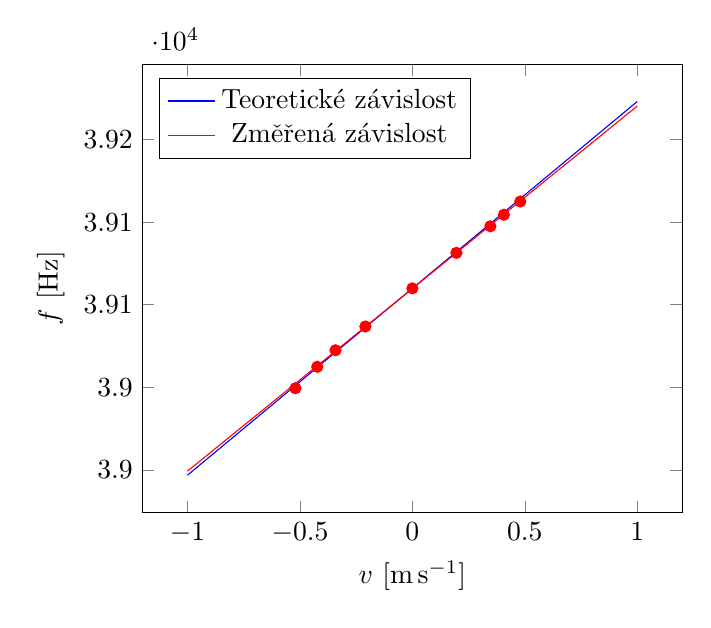
\begin{tikzpicture}
        \begin{axis}[
            xlabel={$v\ [\si{\meter\per\second}]$},
            ylabel={$f\ [\si{\hertz}]$},
            legend pos=north west,
        ]

        \addplot [
          domain = -1:1,
          color = blue,
        ] {113.148*x+39059.9};
        \addlegendentry{Teoretické závislost}

        \addplot [
          domain = -1:1,
          color = red,
        ] {110.556*x+39059.75};
        \addlegendentry{Změřená závislost}

        \addplot[
         color = red,
         mark = *,
         only marks,
        ] coordinates {
         (0, 39059.9)
         (0.196, 39081.4)
         (-0.209, 39036.8)
         (0.347, 39097.5)
         (-0.342, 39022.4)
         (0.407, 39104.5)
         (-0.423, 39012.4)
         (0.480, 39112.5)
         (-0.520, 38999.4)
        };
        \end{axis}
    \end{tikzpicture}
\end{figure}

\newpage
\subsection{Výpočet nejistot}
\begin{equation}
 u_A(f) = \sqrt{\frac{\sum_{i=1}^N (f_i - \bar{f})^2}{N(N-1)}}
\end{equation}
\begin{table}[!ht]
    \centering
    \begin{tabular}{|c|c|}
        $v\ [\si{\meter\per\second}]$ & $u_A(f)\ [\si{\hertz}]$ \\ \hline
        0.000 & 0.180 \\
        0.196 & 0.267 \\
        -0.209 & 0.200 \\
        0.347 & 0.500 \\
        -0.342 & 0.221 \\
        0.407 & 0.307 \\
        -0.423 & 0.427 \\
        0.480 & 1.447 \\
        -0.520 & 0.562 \\
    \end{tabular}
\end{table}

$$\sigma_{a_1} = 0.36$$
\section{Závěr}
Změřili jsme závislost pozorované frekvence na rychlsoti vysílače. Pro porovnání s teoretickou hodnotou využíváme směrnici této závislosti. Ta nám změřená vyšla $a_1 = 110.56 \pm 0.36$ což se od té spočtené $a_1 = 113.15$ liší o 2.3\%.
\end{document}
